\section{Generated parser}

The parser receives tokens from the scanner.
It interprets the grammar derivations.
Upon decoding each derivation, its associated semantic action is executed.
These semantic actions generate the output of the parsing process.
The executable form of the parser can be depicted as follows:
\begin{figure}[H]
    \centering
    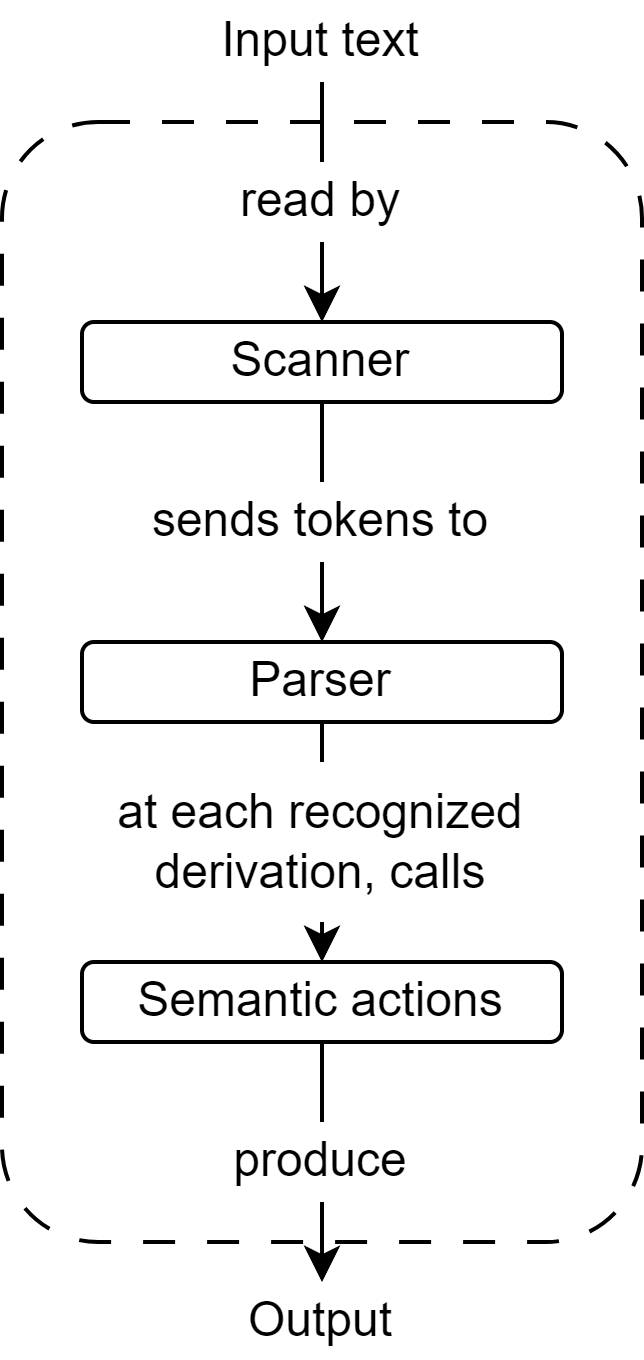
\includegraphics[width=0.2\linewidth]{images/parser.png}
    \caption{Parser executable workflow}
\end{figure}
The generated parser consists of a C file with the extension \texttt{.tab.c} and an accompanying header file with the extension \texttt{.tab.h}. 
The primary parsing function is: \\
\texttt{int yyparse(void);} \\ 
To read tokens, the parser utilizes the same \texttt{yylex()} function provided by FLEX-generated scanners. 
This function is invoked whenever the parser needs a new token.